\chapter{Concept\label{cha:chapter3}}
This chapter outlines the requirements and design choices necessary for developing the RDF Instance Generator Schema Visualizer and the RDF web service.

\section{Overview\label{sec:reqoverview}}

This project aims to simplify RDF schema exploration, validation, and instance generation. To achieve this, the following categories of requirements have been defined:
\begin{itemize}
    \item Functional requirements: Core features such as instance generation, schema validation, and visualization.
    \item Non-functional requirements: Considerations related to performance, usability, and cross-platform compatibility.
    \item Technical requirements: Specifications for the underlying technologies and system design.
    \item Data privacy and security requirements: Measures to ensure the protection and confidentiality of user data.
\end{itemize}

The design prioritizes a client-server architecture and cross-platform compatibility to enhance usability and efficiency. 
\\
The web service is designed to be compatible with various browsers and IDEs. 
\\
The IDE extension will support users and seamlessly integrate into their workflow.

\section{Functional requirements\label{sec:techreq}}
This section covers the functional requirements for the entire system.

\subsection{Instance Generation\label{sec:reqsuba}}
The first requirement for this project is the generation of synthetic RDF instances.
\\
When a user is writing an RDF file—in Turtle, N3, XML, or other RDF formats—the system will generate synthetic RDF instances to save time by avoiding manual insertion of test data.
\\
The application will not only generate compatible RDF triples but will also allow users to modify the automatically generated instances.

\subsection{Schema Validation\label{sec:reqsuba}}
The program should be designed to validate a user-defined RDF schema by checking the structural integrity and semantic consistency of its triples. 
Each triple should conform to syntactic constraints (e.g., proper use of IRIs, literals, and blank nodes), and the asserted relationships should not lead to logical contradictions or unintended inferences.
\\
If errors are found in the schema description, feedback should be provided to the user via the UI or terminal.

\subsection{Multi-Vocabulary Support\label{sec:reqsuba}}
Interoperability and semantic richness are crucial for ensuring seamless data integration, enhancing knowledge representation, and enabling efficient querying and reasoning across diverse RDF datasets.
By supporting multiple vocabularies and ontologies—such as RDFS, FOAF, Schema.org, and others—the system should be able to handle a wide range of RDF data sources and visualize them as graphs.

\subsection{Import and Export\label{sec:reqsuba}}
The software should allow users to import their custom RDF files and export the files with automatically generated instances in the same format.

\subsection{Schema Visualization\label{sec:reqsuba}}
To simplify the exploration and analysis of RDF data from a human perspective, the program should display the RDF schema as a graphical representation.
The displayed graph should support interactive features such as zooming, panning, and collapsing nodes.
\\
The graphical representation should adapt based on schema complexity and hierarchical structure.
\\
In the IDE extension, the user should be able to visualize the graph in a side panel window next to the RDF file they are working on.

\section{Non-functional requirements\label{sec:techreq}}
This section defines the non-functional requirements of the system.

\subsection{Performance\label{sec:reqsuba}}
The system should ensure high-performance rendering of large RDF graphs to support smooth visualization and interaction. Additionally, actions such as node selection and zooming should occur with minimal latency to maintain a responsive user experience. The system should optimize its rendering pipeline to enable real-time exploration of complex RDF schemas without sacrificing performance.

\subsection{Usability\label{sec:reqsuba}}
Both the IDE extension and the web application should feature an intuitive, user-centric interface that enhances accessibility and minimizes the learning curve. To achieve this, the design should incorporate familiar UI elements to ensure a seamless and user-friendly experience.

\subsection{Compatibility\label{sec:reqsuba}}
To ensure smooth integration across different development environments, the web service should be designed for cross-platform compatibility, allowing easy adoption in various IDEs with minimal adjustments. This enhances interoperability, enabling the service to operate consistently across software ecosystems.
\\
To validate this, minor features should also be implemented in a secondary IDE.

\section{Technical Requirements\label{sec:techreq}}

\subsection{Web Architecture\label{sec:reqsuba}}
The system should follow a client-server architecture. While there are no constraints on the specific communication technologies (e.g., SOAP, REST, gRPC), the architecture must follow web principles and use web technologies—such as HTML, CSS, JavaScript, or WebAssembly—and protocols such as HTTP and WebSockets.

\subsection{IDE extension\label{sec:reqsuba}}
The application should be accessible via a web-based client to ensure wide availability. However, the main emphasis should be placed on integration as an extension within widely used IDEs.

\section{Data privacy and Security\label{sec:techreq}}

\subsection{Security\label{sec:reqsuba}}
To ensure the confidentiality and integrity of RDF data, the system should use secure data transmission protocols, such as HTTPS, to protect sensitive information during transfer.

\subsection{Confidentiality\label{sec:reqsuba}}
According to the current design, no data should be stored from the business logic layer. 
\\
All data processing will occur in-memory, either on the client-side or server-side, ensuring that user data is never persistently stored. This ephemeral data handling strategy significantly reduces the risk of data retention and unauthorized access. Consequently, it minimizes compliance obligations related to long-term data storage, such as those outlined in the General Data Protection Regulation (GDPR). 

\section{Solution strategy\label{sec:techreq}}
As stated in the requirements section, the system uses a client-server architecture where the client and server serve distinct roles in the overall functionality.

\begin{figure}[H]
    \centering
    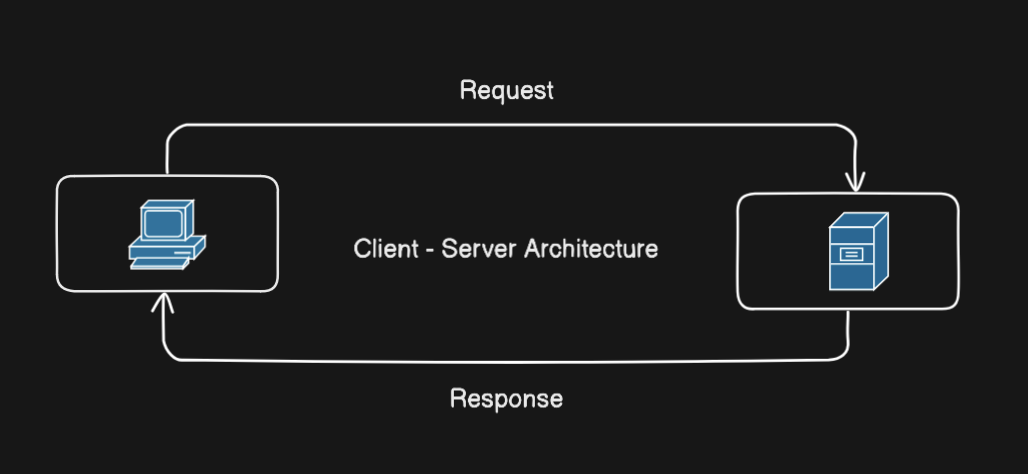
\includegraphics[width=14cm]{client_server.png}\\
    \caption{Client / Server}\label{fig:client_server}
\end{figure}

\subsection{Client\label{sec:reqsuba}}
To ensure broad system availability, the system is designed to support two types of user agents:
\begin{itemize}
    \item Browsers
    \item Integrated Development Environments 
\end{itemize}
The browser selected by the user should access the web application via the HTTP protocol.
The user will then upload their RDF file and send it to the server.
The client will receive the processed information and display the resulting graph (see Figure \ref{fig:BrowserGraphView}).

\begin{figure}[htb]
    \centering
    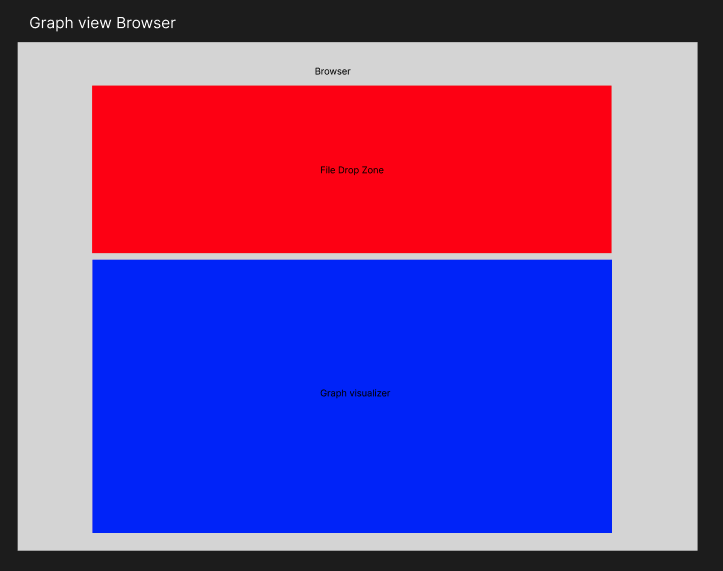
\includegraphics[width=14cm]{mock dropzone.png}\\
    \caption{Browser file drop zone and graph view}\label{fig:BrowserGraphView}
\end{figure}

Additionally, the user should be able to view the RDF file alongside the generated instances and its graphical representation (see Figure \ref{fig:BrowserRDFReader}).

\begin{figure}[htb]
    \centering
    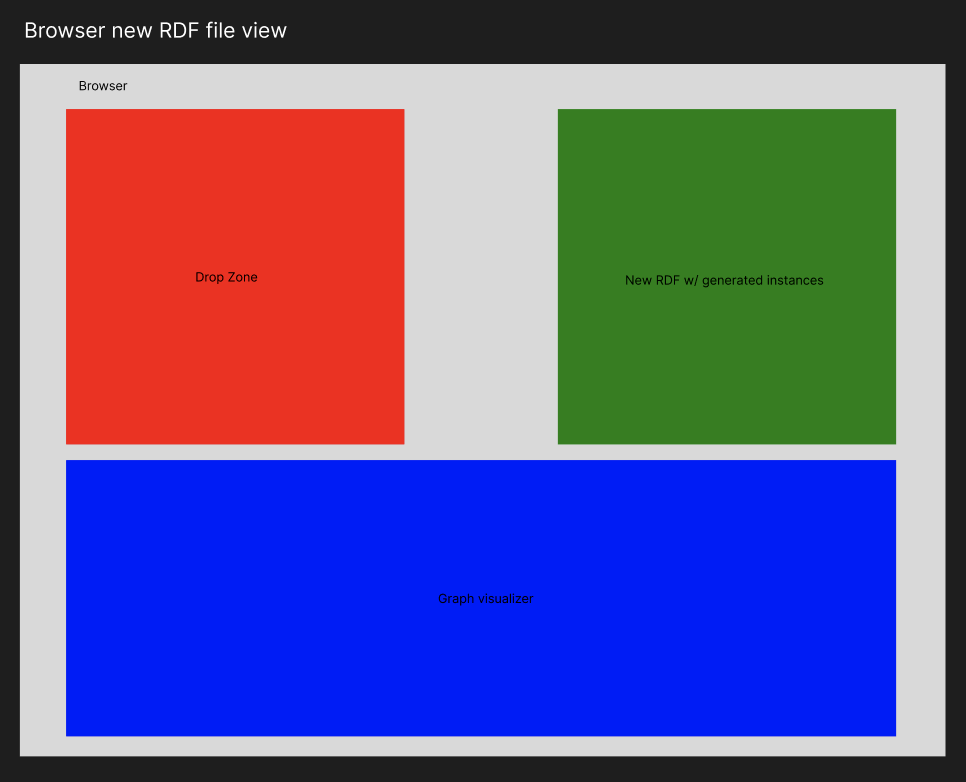
\includegraphics[width=14cm]{mock_browser_new_RDF_instance.png}\\
    \caption{Browser new RDF side panel view}\label{fig:BrowserRDFReader}
\end{figure}

Within the IDE, the user experience will be slightly different from the browser. Instead of uploading an RDF file, users will interact with the system directly in the IDE. While working on an RDF file and executing a predefined command, a web-based visualization panel will dynamically open beside the file, rendering an interactive graphical view of the RDF schema in real time. This allows users to examine relationships, structures, and dependencies without leaving their coding environment (see Figure \ref{fig:IDEGraphView}). 

\begin{figure}[H]
    \centering
    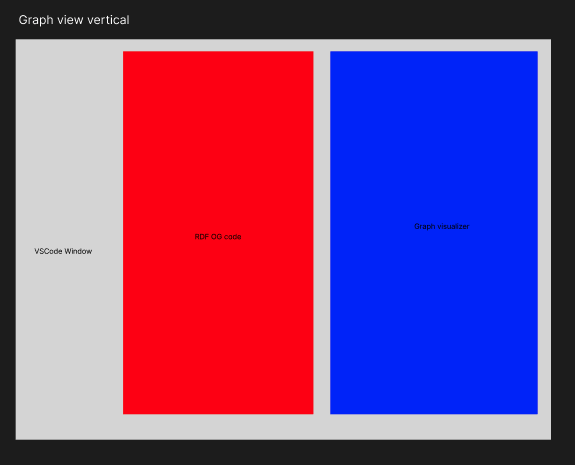
\includegraphics[width=14cm]{mockup side panel view.png}\\
    \caption{IDE Graph side panel view}\label{fig:IDEGraphView}
\end{figure}

The extension will not only support the visualization of RDF files in user-specified formats—like its browser counterpart—but will also allow real-time editing of the file (see Figure \ref{fig:IDERDFReader}).

\begin{figure}[htb]
    \centering
    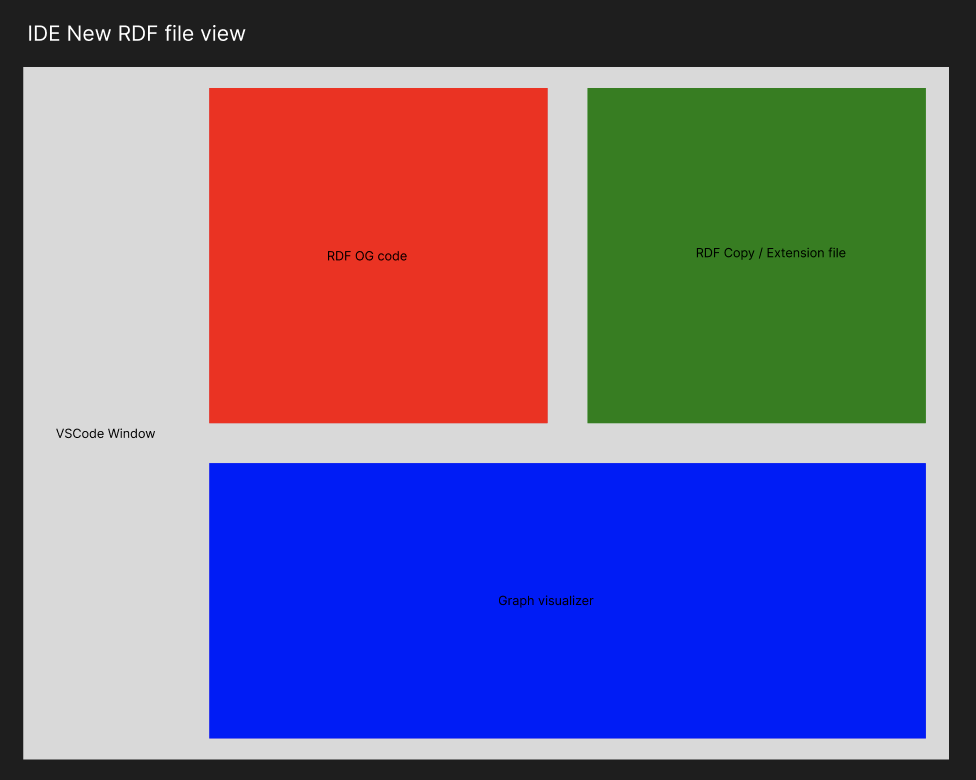
\includegraphics[width=14cm]{mock_ide_new_RDF_instance.png}\\
    \caption{IDE new RDF side panel view}\label{fig:IDERDFReader}
\end{figure}

\subsection{Server\label{sec:server}}
To ensure system compatibility across various devices, operating systems, and user agents, the server is responsible for all computational tasks and data processing. By centralizing calculations and RDF graph handling on the server side, the system reduces client-side resource use and improves performance consistency.
\\
\\
The server plays a critical role in managing RDF data—ensuring schema validation, instance generation, SPARQL query processing, and graph construction.
\\
Upon receiving an RDF file, the server scans it for potential flaws, such as syntactic or semantic errors. It should be capable of handling multiple RDF serialization formats, including Turtle, N3, XML, and JSON-LD.
\\
\\
The service generates synthetic RDF instances based on the given schema, maintaining logical consistency with the original data.
\\
It identifies RDF classes and properties and creates additional instances where necessary to preserve semantic correctness.
\\
This is particularly important when a property references an instance of a class that hasn’t been explicitly defined. For example, if a schema includes a `hasCar` property that expects an instance of the `Car` class, the system will automatically generate one if it does not exist. This maintains logical coherence and satisfies all property constraints. By dynamically generating required instances, the system preserves data integrity, prevents incomplete assertions, and supports reliable reasoning processes in RDF applications.
\\
The additional generated instances should have realistic properties and values that meet graph constraints.
\\
\\
Finally, the service returns the newly generated RDF file in the requested format, along with its graphical representation.
